\documentclass[11pt,a4paper]{article}
\usepackage{fullpage}
\usepackage[utf8]{inputenc} % For å kunne skrive norske tegn.
\usepackage{graphicx} % For å inkludere figurer.
\usepackage{amsmath,amssymb} % Ekstra matematikkfunksjoner.
\usepackage[]{algorithm2e}
\usepackage{listings}
\usepackage{enumitem}
\usepackage{caption}
\usepackage{subcaption}
\setlist{nosep}


\author{Jon Christian Halvorsen and Anders Opskar Voldsund}
\title{ \textbf{ AI Programming Project Module \# 6 }  \\
Deep Learning for Game Playing }
\date{\today}

\begin{document}
\maketitle

\section*{Designing Our ANN}
For this module we based our ANN on our best ANN from the previous module. We used the sigmoid function as activation function and least squares as error function. For our net we used one layer with 12 nodes. We noticed that a learning rate of 0.2 worked well for our situation. The percentage of correct moves for this ANN gave around 40 $\%$, which we thought statistically significant compared to a random player with an average of 25 $\%$ correct moves.

\section*{Generating Training Data}
To generate our training data we ran our old 2048 algorithm, but only recorded data for every game which obtained a highest tile above or equal to 1024. For these games we saved every state and every move performed, until we had above 100 000 different states and different moves. This resulted in 101 221 different states where the percentage of moves are recorded in Table \ref{tab:percantage}.

\begin{table}[h!]
\centering
\caption{Move percentages for the training data}
\begin{tabular}{cc}
move & percentage \\
\hline
left & 28.3 $\%$ \\
up & 24.9 $\%$ \\
right & 21.5 $\%$ \\
down & 25.3 $\%$
\end{tabular}
\label{tab:percantage}
\end{table}

\section*{Two Different Representations}
The two representations that we attempted are given below. We ran each of them 50 times and used Welch's T-test to justify which was the better.

\subsection*{Representation I}
In our first representation we simply represented each game state as a vector of length 16, where each element corresponded to the value on the board divided by some number. We chose 255 as this number (we also tried with 256, but seemed to get better results using 255. We have no idea why). The idea is that we want to map the values to the range (0,1). As our neural network quite consistently give values of maximum 256, with some exceptions, we get all these values in the desired range. An example transformation is shown below:

\begin{align*}
\begin{pmatrix}
  2  &  4 &   8 &  4\\
  2  &  8 &  16 & 32 \\
  8  & 16 &  64 & 128 \\
  16 & 64 & 256 & 512
\end{pmatrix}
\rightarrow
\frac{1}{255}
\begin{pmatrix}
  2  &  4 &   8 &  4\\
  2  &  8 &  16 & 32 \\
  8  & 16 &  64 & 128 \\
  16 & 64 & 256 & 512
\end{pmatrix}
\end{align*}

\subsection*{Representation II}
In our second representation we take our vector of length 16, and take $\textrm{log}_2$ of every element. As our neural network usually gives values up to 256, we choose to divide every element by 8, as $\textrm{log}_2(256) = 8$. This will map all elements below or equal to 256 in the range (0,1). An example transformation is given below:

\begin{align*}
\begin{pmatrix}
  2  &  4 &   8 &  4\\
  2  &  8 &  16 & 32 \\
  8  & 16 &  64 & 128 \\
  16 & 64 & 256 & 512
\end{pmatrix}
\rightarrow
\frac{1}{8}
\begin{pmatrix}
  1 & 2 & 3 & 2 \\
  1 & 3 & 4 & 5 \\
  3 & 4 & 6 & 7 \\
  4 & 6 & 8 & 9
\end{pmatrix}
\end{align*}

\subsection*{Comparing Representation I and II}
We performed 50 runs of the ANN-based player with representation I and II, as well as 50 runs of the random player. For these 50 runs, the random player averaged a maximum tile of 102.4. Representation I achieved an average maximum tile of 225, while representation II achieved an average maximum tile of 151.

Representation I gave  



\section*{Analysis Of A 2048 Game}
We chose to take a closer look at one of the games played using representation I. In the first sequence of moves (as illustrated in figure \ref{fig:first_seq}) we see what may look like a stupid move in the start; not merging downwards so we get a 4-2-4 pattern. Although this move may seem stupid, it works out great, and at the end of the sequence we have a (quite) optimal tile placement.

\begin{figure}[h!]
    \centering
    \begin{subfigure}[b]{0.22\textwidth}
        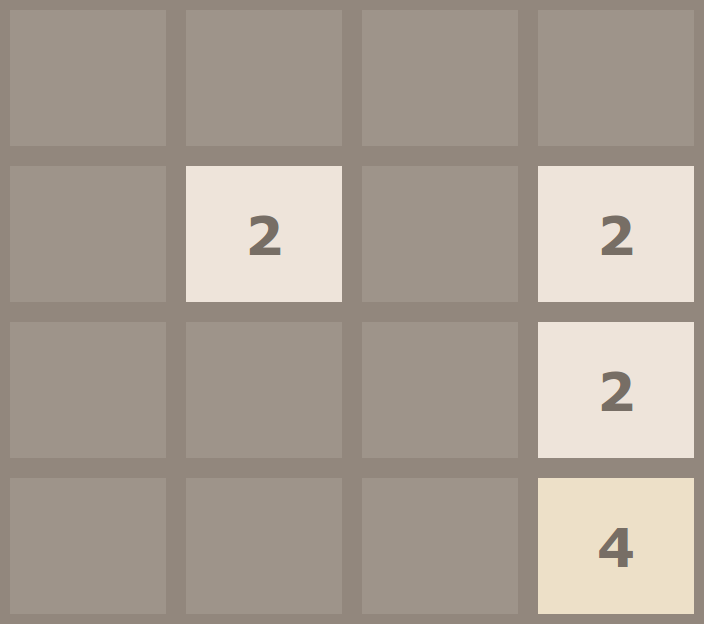
\includegraphics[width=\textwidth]{figures/1}
    \end{subfigure}
    ~
    \begin{subfigure}[b]{0.22\textwidth}
        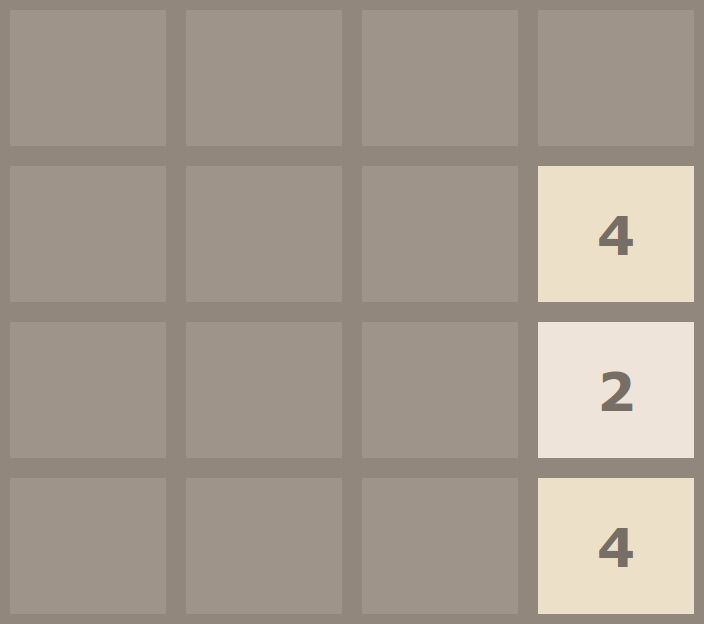
\includegraphics[width=\textwidth]{figures/2}
    \end{subfigure}
    ~
    \begin{subfigure}[b]{0.22\textwidth}
        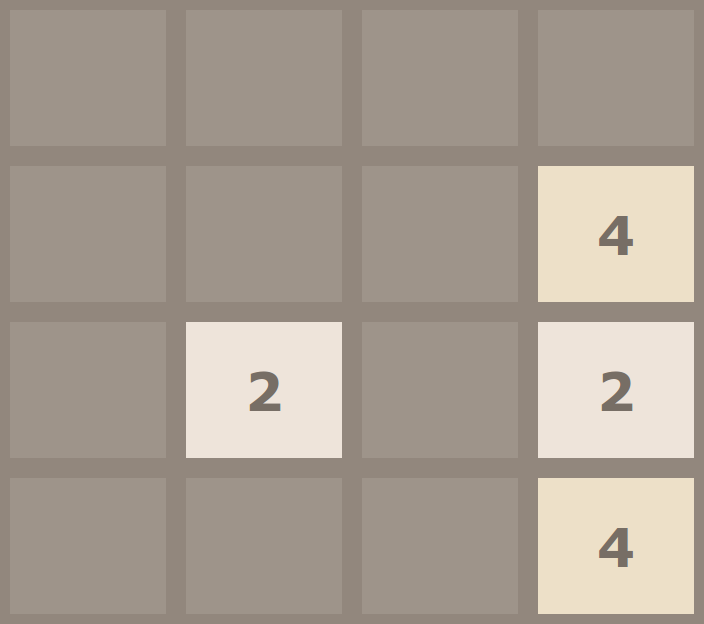
\includegraphics[width=\textwidth]{figures/3}
    \end{subfigure}
    ~
    \begin{subfigure}[b]{0.22\textwidth}
        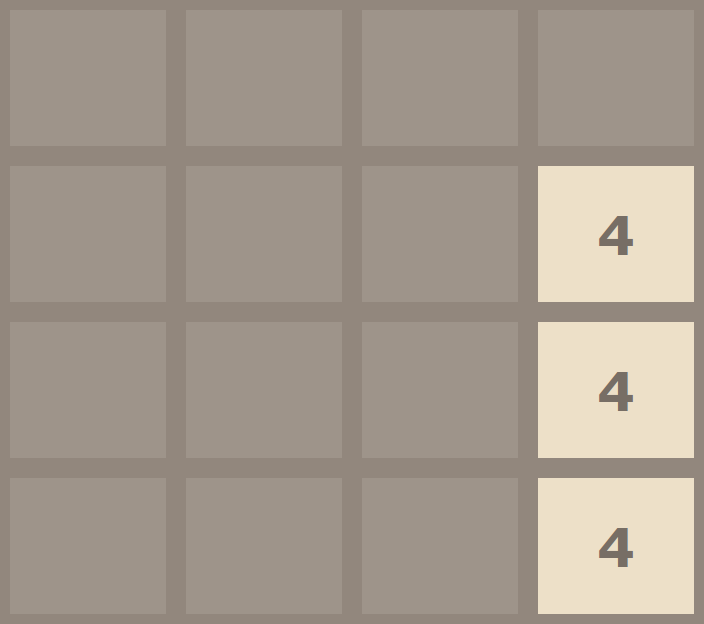
\includegraphics[width=\textwidth]{figures/4}
    \end{subfigure}
    \vfill
    \begin{subfigure}[b]{0.22\textwidth}
        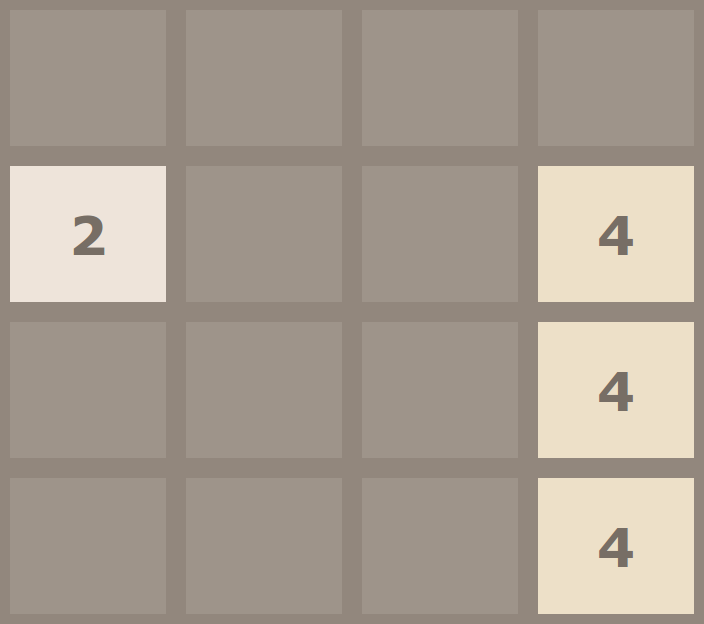
\includegraphics[width=\textwidth]{figures/5}
    \end{subfigure}
    ~
    \begin{subfigure}[b]{0.22\textwidth}
        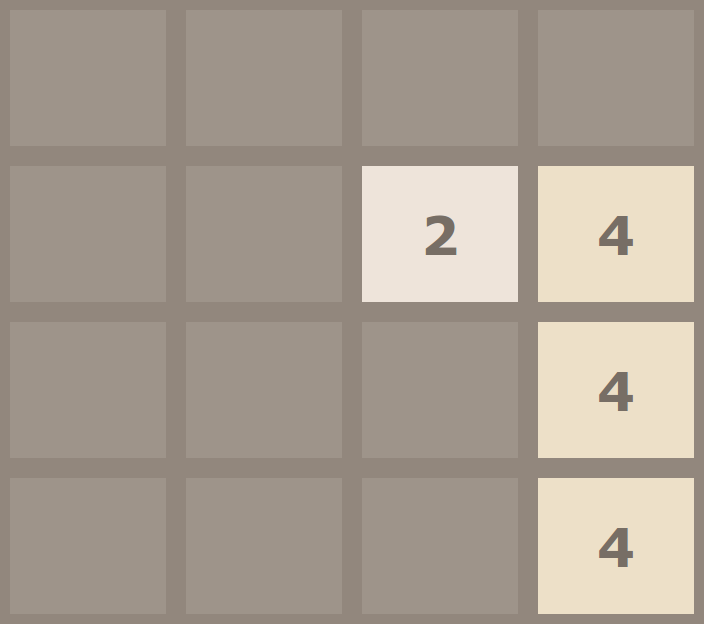
\includegraphics[width=\textwidth]{figures/6}
    \end{subfigure}
    ~
    \begin{subfigure}[b]{0.22\textwidth}
        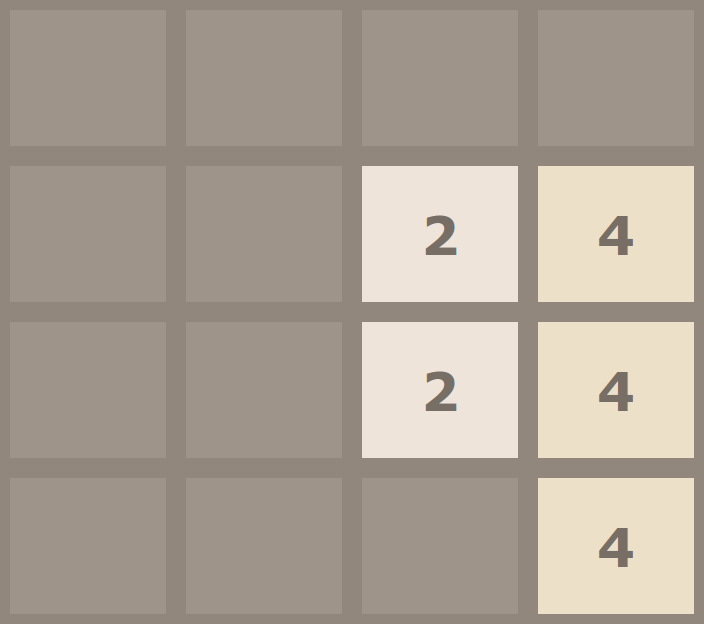
\includegraphics[width=\textwidth]{figures/7}
    \end{subfigure}
    ~
    \begin{subfigure}[b]{0.22\textwidth}
        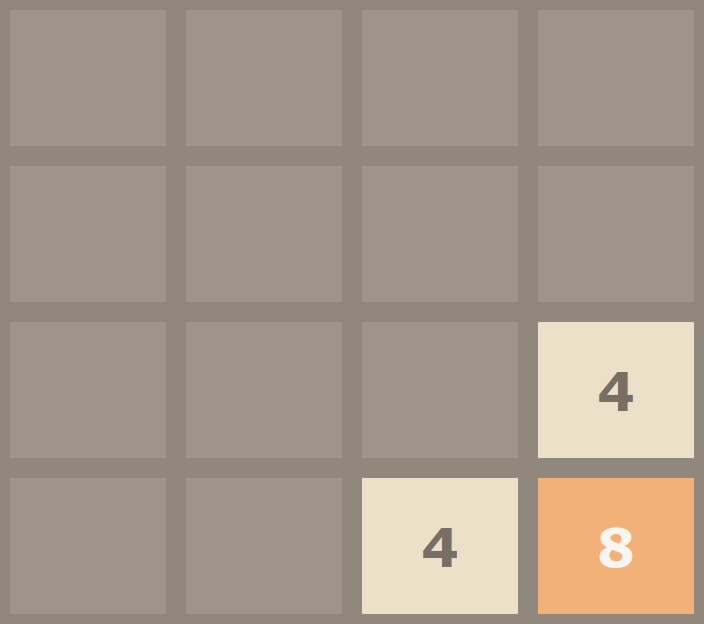
\includegraphics[width=\textwidth]{figures/8}
    \end{subfigure}
    \caption{First sequence of moves from our neural network playing 2048.}
    \label{fig:first_seq}
\end{figure}

In our second example (as illustrated in figure \ref{fig:second_seq}) the neural net decide that it is advantageous to merge the two 64-tiles to get a 128-tile. This means however that we are stuck with a 2-tile between an 8-tile and the 128 tile. This in fact leads to the game ending quite soon after. We're not quite sure how we could have fixed this problem here, but our old search-bases algorithm would probably never chose a path in the searchtree that would end this way.

\begin{figure}[h!]
    \centering
    \begin{subfigure}[b]{0.45\textwidth}
        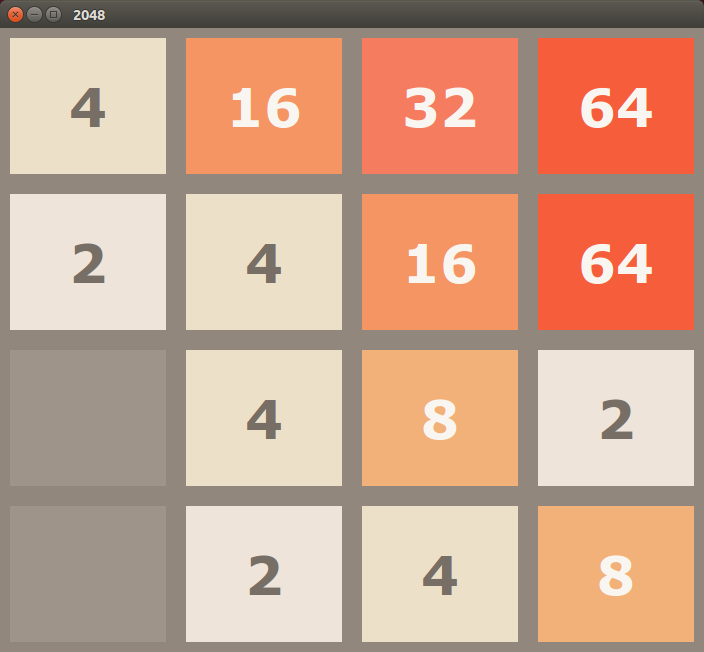
\includegraphics[width=\textwidth]{figures/64}
    \end{subfigure}
    ~
    \begin{subfigure}[b]{0.45\textwidth}
        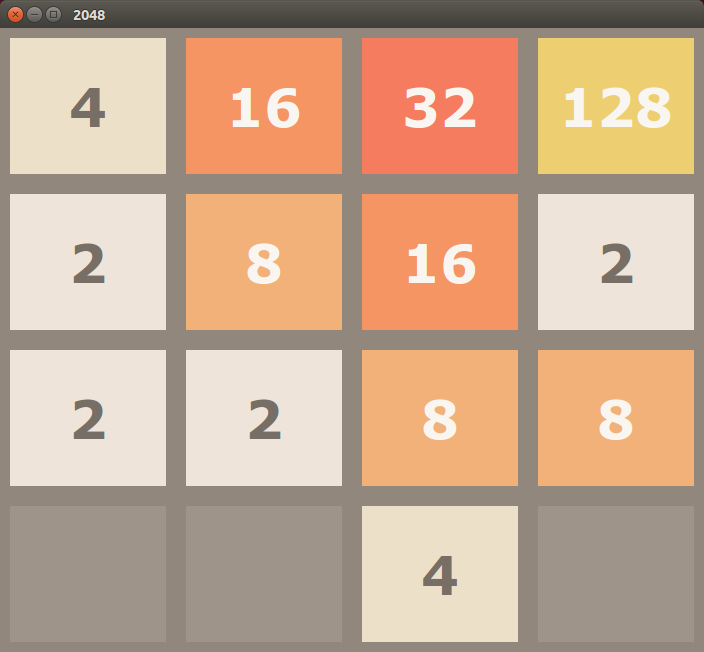
\includegraphics[width=\textwidth]{figures/128}
    \end{subfigure}
    \caption{Second sequence of moves from our neural network playing 2048.}
    \label{fig:second_seq}
\end{figure}


\end{document}